\chapter{动力学平均场理论(DMFT)}
动力学平均场理论(Dynamical Mean Field Theory, DMFT)的核心思想是将晶格模型自洽地映射为单杂质量子模型,将难以求解的晶格问题转化成量子杂质问题,从而有效降低多体问题的自由度。在处理量子杂质模型时,由于杂质哈密顿量并不会因为晶格模型的不同类型而发生较大变化,因此这一方法的优势是可以处理不同的晶格问题,可以进一步与真实的材料体系计算相结合,很大程度上扩展了强关联材料的计算领域。
\section{模型映射}
为了将晶格模型的性质映射到单杂质模型中,一个直接的方式是扣除晶格模型的一个格点,利用路径积分将其他格点积分掉,得到与单杂质模型数学形式相同的有效作用量。文献中一般称这种推导方法为空腔法(cavity method)\cite{RevModPhys.68.13}。下面从经典 Ising 模型出发,简要介绍空腔法的思路,并具体推导由 Hubbard 模型到单杂质 Anderson 模型的映射。
\subsection{Ising model}
首先以经典 Ising 模型为例, 推导空腔的有效哈密顿量。 Ising 模型的哈密顿量为 
\begin{equation}
    \begin{aligned}
        H=&-\sum_{\langle ij \rangle}J_{ij}S_iS_j-h\sum_iS_i\\
        \equiv&-h_oS_o-\sum_i J_{io}S_oS_i+H^{(o)},
    \end{aligned}
\end{equation}
其中 $J_{ij}>0$ 是最近邻铁磁相互作用, $\sum_{\lag ij \rag}$ 是对最近邻格点对求和, 自旋取 $S_i=\pm 1$。式中第二行将哈密顿量分成三项: 第一项是挖去一个格点 $o$ 之后, $o$ 格点的哈密顿量 $H_o$。第二项是 $o$ 与格点的耦合项 $\Delta H$, 格点周围剩余的格点称为空腔, 哈密顿量是式中第三项 $H^{(o)}$。空腔法的模型如图所示。
\begin{figure}[H]
    \vspace{13pt} % 调整图片与上文的垂直距离
    \centering
    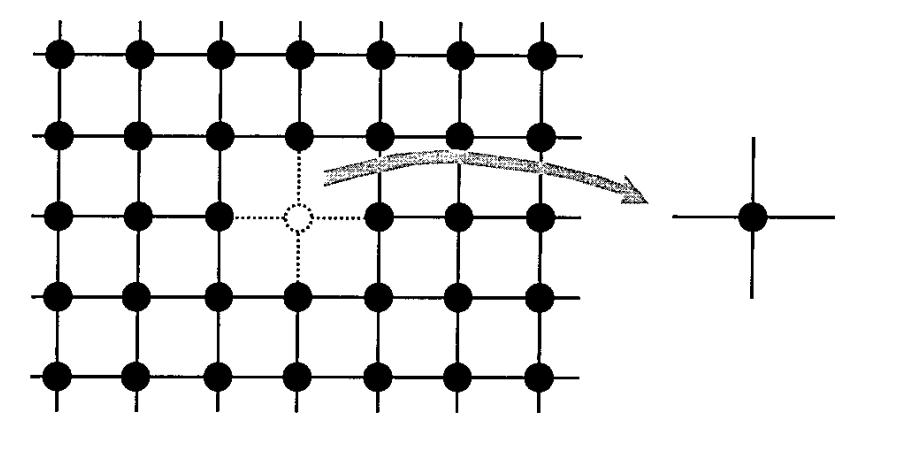
\includegraphics[width=5in]{Img/cavity-method.png}
    \caption{在格点模型中挖去一个格点 $o$ 以及 $o$ 和其他格点的相互作用键} 
\end{figure}
定义作用在格点 $i$ 上的场 $\eta_i$:
\begin{equation}
    \eta_i\equiv J_{io}S_o,
\end{equation}
于是哈密顿量可以改写为 
\begin{equation}
    \left\{
        \begin{aligned}
            H&=H_o+H^{(o)}+\Delta H,\\
            H_o&=-h_oS_o,\\
            \Delta H&=-\sum_{i\ne o}J_{io}S_oS_i\equiv\sum_i\eta_iS_i.
        \end{aligned}
    \right.
\end{equation}
利用有效密度矩阵, 把所有非零格点求迹掉, 从而定义 $o$ 格点的有效哈密顿量:
\begin{equation}
    \e^{-\beta H_o^{\fun{eff}}[S_o]}\equiv \sum_{\{ S_i \}\atop i\ne 0}\e^{-\beta H}.
\end{equation}
其中, 对 $S_i$ 的求和可以得到空腔哈密顿量 $H^{(o)}$ 关联函数的生成泛函, 对上式两边求关于 $\eta_i$ 的各阶导, 可以得到 $\hoeff$ 的各阶导数。然后代入到 $H_o^{\fun{eff}}[S_o]$ 的展开式
\begin{equation}
    H_o^{\fun{eff}}[S_o]=\left. H_o^{\fun{eff}}[S_o]\right|_{\{\eta_i=0\}} +\left.\sum_i\frac{\pt H_o^{\fun{eff}}}{\pt \eta_i}\right|_{\{\eta_i=0\}}\eta_i+\cdots,
\end{equation}
就能得到有效哈密顿量的具体形式。下面逐阶计算各阶导数。

(i) 一阶导:
\begin{equation}
    \begin{aligned}
        -\beta \e^{-\beta H_o^{\fun{eff}}}\cdot \frac{\pt \hoeff}{\pt \eta_i}=&-\beta \sum_{\{S_j\}\atop j\ne o}\lmi -S_i\e^{-\beta\ls -h_oS_o-\sum_{k\ne o}\eta_kS_k+H^{(o)} \rs} \rmi\\
        \Rightarrow \left.\frac{\pt \hoeff}{\pt \eta_i}\right|_{\{\eta_i=0\}}=&\left.-\frac{\sum_{S_j\atop j\ne o}\lmi -S_i\e^{-\beta(-h_oS_o-\sum_k\eta_kS_k+H^{(o)})} \rmi}{\sum_{\{S_j\}\atop j\ne o}\e^{-\beta\lmi -h_o S_o-\sum_k \eta_kS_k +H^{(o)} \rmi}}\right|_{\{\eta_i=0\}}\\
        =&-\frac{\sum_{\{S_j\}\atop j\ne o}S_i\e^{-\beta H^{(o)}}}{\sum_{\{S_j\}\atop j\ne o}\e^{-\beta H^{(o)}}}\\
        = &-\lag S_i \rag_{H^{(o)}}\\
        \equiv & -\lag S_i \rag_o,
    \end{aligned}
\end{equation}
对 $\eta_i$ 积分一次, 得到:
\begin{equation}
    \hoeff|_{\{\eta_i=0\}} = C-h_o\lag S_i \rag_o.
\end{equation}

(ii) 二阶导:
\begin{equation}
    -\beta\e^{-\beta\hoeff}\frac{\pt^2\hoeff}{\pt \eta_{i_1}\pt\eta_{i_2}}+\beta^2\e^{-\beta\hoeff}\frac{\pt\hoeff}{\pt\eta_{i_1}}\frac{\pt\hoeff}{\pt \eta_{i_2}}=\beta^2\sum_{\{S_j\}\atop j\ne o}\lmi S_{i_1}S_{i_2}\e^{-\beta\ls -h_o S_o+H^{(o)}-\sum_k \eta_k S_k \rs} \rmi,
\end{equation}
整理得到:
\begin{equation}
    \begin{aligned}
        \frac{\pt^2 \hoeff}{\pt\eta_{i_1}\pt\eta_{i_2}}=\beta\frac{\pt\hoeff}{\pt\eta_{i_1}}\frac{\pt\hoeff}{\pt\eta_{i_2}}-\frac{\beta\sum_{\{S_j\}\atop j\ne o}\lmi S_{i_1}S_{i_2}\e^{-\beta\ls -h_oS_o+H^{(o)}-\sum_k\eta_k S_k \rs} \rmi}{\sum_{\{S_j\}\atop j\ne o}\e^{-\beta\ls -h_oS_o-\sum_k\eta_k S_k+H^{(o)} \rs}},
    \end{aligned}
\end{equation}
将一阶导的结果带入上式, 有
\begin{equation}
    \left.\frac{\pt^2\hoeff}{\pt\eta_{i_1}\pt \eta_{i_2}}\right|_{\eta_i=0}=\beta\lag S_{i_1} \rag_o\lag S_{i_2} \rag_o-\beta\lag S_{i_1}S_{i_2} \rag_o\equiv -\beta\lag S_{i_1}S_{i_2} \rag_o^{\fun{c}},
\end{equation}
其中期望值的上标 $\fun{c}$ 表示连接的关联函数(linked correlated function)。

利用类似方法, 可以得到各阶导数与挖去 $o$ 格点后的关联函数之间的关系为 
\begin{equation}
    \left. \frac{\pt^n\hoeff}{\pt\eta_{i_1}\cdots \pt\eta_{i_n}} \right|_{\eta_i=0}=-\beta^{n-1}\lag S_{i_1}\cdots S_{i_n} \rag_o^{\fun{c}},
\end{equation}
将上式代入 $\hoeff$ 的泰勒展开式中, 可以在形式上得到: 
\begin{equation}
    \hoeff [S_o]=C-h_oS_o+\sum_{n=1}^{\infty}\frac{-\beta^{n-1}}{n!}\sum_{i_1\cdots i_n\atop (1,\cdots,n\ne o)}\lag S_{i_1}\cdots S_{i_n} \rag_o^{\fun{c}}\eta_{i_1}\cdots \eta_{i_n}.
\end{equation} 
为了在维度 $D\to \infty$ 时得到有限的临界温度, 人们证明了, 需要对耦合强度作标度变换:
\begin{equation}
    J_{ij}=\frac{\tilde{J}}{D^{|i-j|}},
\end{equation}
其中 $\tilde{J}$ 是不随维数变化的一个常数, $|i-j|$ 表示两格点之间的 Manhattan 距离, 此 "距离" 只能沿格点计数, 例如下图中 $|i-j|=2$, $|k-l|=4$。
\begin{figure}[H]
    \vspace{13pt} % 调整图片与上文的垂直距离
    \centering
    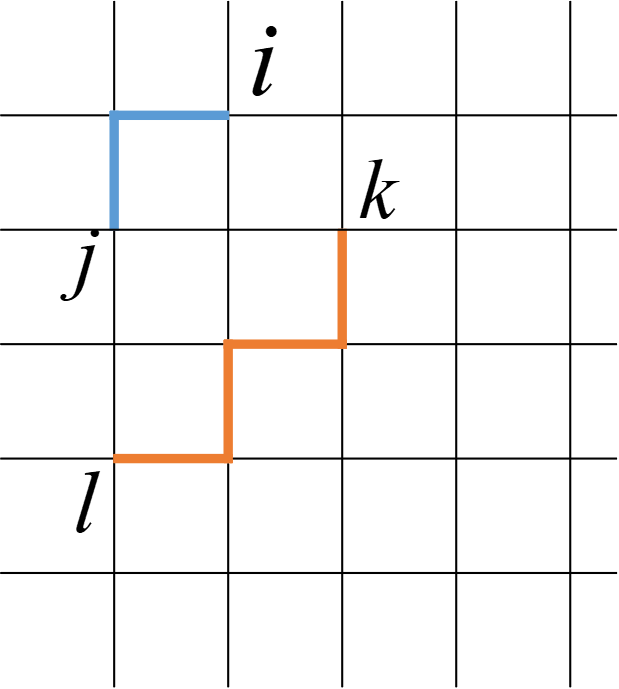
\includegraphics[width=3in]{Img/manhattan.png}
    \caption{Manhattan 距离的示意图。} 
\end{figure}
% 下面考虑 \eqref{Heff-taylor} 各项展开式中 $D$ 的阶数.
% \par $n=1$ 时: 
% \begin{equation}
%     -\sum_{i\ne o}\lag S_i \rag_oJ_{io}S_o\sim \frac{\tilde{J}_1}{D}D+\frac{\tilde{J}_2}{D^2}D^2+\cdots
% \end{equation}
可以证明, 当 $D\to \infty$ 时, 只有 $n=1$ 项保留, 高阶项为零。有效哈密顿量可以表示为
\begin{equation}
    \hoeff [S_o]= -h S_o-\sum_{i\ne o}J_{oi}\lag S_i \rag^{(o)}.
\end{equation}
从中可以定义有效场 $h_{\fun{eff}}$:
\begin{equation}
    h_{\fun{eff}}=h+\sum_{i\ne o}J_{oi}\lag S_i \rag^{(o)},\quad \hoeff =-h_{\fun{eff}}S_o.
\end{equation}
考虑到格点的平移不变性 $\lag S_o \rag=\lag S_i \rag$ 后, 这一结果与 Weiss 平均场理论一致。

\subsection{Hubbard model}
下面考虑量子情形。

Hubbard 模型的哈密顿量为
\begin{equation}
    \hat{H}=-\sum_{ij\sigma}t_{ij}^{ }c_{i\sigma}^\dg c_{j\sigma}^{ }+U\sum_i n_{i\ua} n_{i\da},
\end{equation}
其中, 设 $t_{ii}=0$, $t_{ij}=t_{ji}\in \mathbb{R}$。

在相干态路径积分下, 有配分函数 
\begin{equation}
    Z=\int\prod_{i}\prod_\sigma \mathcal{D}c_{i\sigma}^*(\tau)\mathcal{D}c_{j\sigma}^{ }(\tau)\e^{-S},
\end{equation}
其中作用量的表达式为
\begin{equation}
    S=\int_0^\infty\dd\tau\lmi \sum_{i\sigma}c_{i\sigma}^*(\tau)\ls \frac{\pt}{\pt \tau}-\mu \rs c_{i\sigma}(\tau)-\sum_{ij}\sum_\sigma t_{ij}c_{i\sigma}^*(\tau)c_{j\sigma}^{ }(\tau)+U\sum_i n_{i\ua}(\tau)n_{i\da}(\tau) \rmi,
\end{equation}
将作用量划分为空腔 $o$ 格点项 $S_o$, 剩余格点项 $S^{(o)}$ 以及相互作用项 $\Delta S$, 其中 
\begin{equation}
    S_o=\int_0^\beta\dd\tau\lmi \sum_\sigma c_{o\sigma}^*(\tau)\ls \frac{\pt}{\pt \tau}-\mu \rs c_{o\sigma}^{ }(\tau)+Un_{o\ua}(\tau)n_{o\da}(\tau) \rmi,
\end{equation}
\begin{equation}
    \Delta S=-\int_0^\beta \dd\tau\sum_{i\sigma}t_{io}\lmi c_{i\sigma}^*(\tau)c_{o\sigma}^{ }(\tau)+c_{o\sigma}^*(\tau)c_{i\sigma}^{ }(\tau) \rmi.
\end{equation}
记 $\eta_{i\sigma}(\tau)\equiv t_{io}c_{o\sigma}(\tau)$, 并对 $t_{ij}$ 作标度变换:
\begin{equation}
    t_{ij}=\frac{\tilde{t}_{ij}}{D^{\frac{|i-j|}{2}}}.
\end{equation}
这里的标度变换方式与 Ising 模型的处理不同, D. Vollhardt 证明, 这样的取法可以在大维度极限 $D\to \infty$ 时得到有限的 $\lag H_T \rag$, 否则将发散或趋于零\cite{PhysRevLett.62.324}。

定义空腔格点的有效作用量:
\begin{equation}
    \frac{1}{Z_{\fun{eff}}}\e^{-S_{\fun{eff}}}\equiv \frac{1}{Z}\int\prod_{i\ne o}\prod_{\sigma}\mathcal{D}c_{i\sigma}^*\mathcal{D}c_{i\sigma}^{ }\e^{-S},
\end{equation}
为方便表述, 令 $\eta_1^*,\cdots,\eta_{N}^*\equiv \eta_{N+1},\cdots,\eta_{2N}$, 视为和 $\eta_1,\cdots,\eta_{N}$ 相互独立的变量。利用 Grassmann 函数的泰勒展开式:
\begin{equation}
    \begin{aligned}
        S_{\fun{eff}}(\eta_{1},\cdots,\eta_{2N})=&\int\dd\tau L_{\fun{eff}}\\
        =&\int\dd\tau\sum_{n=0}^\infty\sum_{i_1\cdots i_n=1}^{2N}\frac{1}{n!}\left.\frac{\pt^n L_{\fun{eff}}}{\pt\eta_{i_1}\cdots\pt \eta_{i_n}}\right|_{\{\eta_1,\cdots,\eta_{2N}=0\}}\eta_{i_n}\cdots\eta_{i_1},
    \end{aligned}
\end{equation}
利用 
\begin{equation}
    \frac{\pt \eta_{i\sigma}(\tau)}{\pt \eta_{j\sigma'}(\tau')}=\delta_{ij}\delta_{\sigma\sigma'}\delta(\tau-\tau')
\end{equation}
以及有效作用量的定义式, 可以计算各阶偏导数的表达式:
\begin{equation}
    \begin{aligned}
        -\e^{-S_{\fun{eff}}}\int\dd\tau\frac{\pt L_{\fun{eff}}}{\pt \eta_{i_1\sigma}}&=\int\prod_{k\ne o}\prod_\sigma\mathcal{D}c_{k\sigma}^*\mathcal{D}c_{k\sigma}^{ }\e^{-S}\lmi -\int\dd\tau c_{i_1\sigma}^*\rmi\\
        \Rightarrow \int\dd\tau\lmi \e^{-S_{\fun{eff}}}\frac{\pt L_{\fun{eff}}}{\pt \eta_{i_1}} \rmi &=\int\dd\tau\lmi \int\prod_{k\ne o}\prod_\sigma\mathcal{D}c_{k\sigma}^*\mathcal{D}c_{k\sigma}^{ }\e^{-S} c_{i_1\sigma}^* \rmi,
    \end{aligned}
\end{equation}
从中得到 
\begin{equation}
    \begin{aligned}
        \left.\frac{\pt L_{\fun{eff}}}{\pt \eta_{i_1}}\right|_{\{\eta_{1,\cdots,N},\eta_{1,\cdots,N}^*=0\}}=&\frac{\int\prod_{k\ne o}\prod_{\sigma}\mathcal{D}c_{k\sigma}^*\mathcal{D} c_{k\sigma}^{ }\e^{-S^{(o)}}c_{i_1\sigma}^*}{\int\prod_{k\ne o}\prod_{\sigma}\mathcal{D}c_{k\sigma}^*\mathcal{D} c_{k\sigma}^{ }\e^{-S^{(o)}}}\\
        =&\lag c^*_{i_1\sigma}(\tau_{i_1}) \rag^{(o)},
    \end{aligned}
\end{equation}
但是奇数阶 Grassmann 变量的期望值都是 0, 所以这里得到的一阶导为零。再求一次导, 得到 
\begin{equation}
    \begin{aligned}
        \left.\frac{\pt^2 L_{\fun{eff}}}{\pt \eta_{i_1}^{ }\pt \eta_{j_1}^*}\right|_{\{\eta_{1,\cdots,N},\eta_{1,\cdots,N}^*=0\}}&=-\left.\frac{\pt^2 L_{\fun{eff}}}{\pt \eta_{i_1}^{*}\pt \eta_{j_1}^{ }}\right|_{\{\eta_{1,\cdots,N},\eta_{1,\cdots,N}^*=0\}}\\
        &=- \lag c_{j_1\sigma}^{ }(\tau_{j_1})c_{i_1\sigma}^*(\tau_{i_1}) \rag^{(o)}\\
        &=-G^{(o)}(\tau_{j_1},\tau_{i_1}).
    \end{aligned}
\end{equation}
同理, 应有
\begin{equation}
    \left.\frac{\pt^{2n}L_{\fun{eff}}}{\pt\eta_{j_1\sigma}^*\cdots\pt\eta_{j_n}^*\pt \eta_{i_1}^{ }\cdots\pt \eta_{i_n}^{ }}\right|_{\{\eta_{1,\cdots,N},\eta_{1,\cdots,N}^*=0\}}=(-1)^nG^{(o)}(\tau_{j_1}\cdots\tau_{j_n},\tau_{i_1}\cdots\tau_{i_n}).
\end{equation}
在 Taylor 展开式中, 首先, 只考虑 $\eta\eta^*$ 耦合, 不考虑 $\eta\eta$ 和 $\eta^*\eta$ 耦合, 其次, $2n$ 个 Grassmann 变量换序时会产生符号变化 $(-1)^n$ 与上式的符号抵消, 最后, 对应每一阶 $n$, 确定了 $i_1,\cdots,i_n,j_1,\cdots,j_n$ 的取值后, 应有 $n!$ 种排列组合方式, 写成正规形式后可以合并为一项。这样, 展开式可以表示为
\begin{equation}
    \begin{aligned}
        S_{\fun{eff}}=&\sum_{n=0}^\infty \sum_{\lag i_1,\cdots,i_n=1 \rag}^N\sum_{\lag j_1,\cdots,j_n=1 \rag}^N\int \left.\frac{\pt^{2n} L_{\fun{eff}}}{\pt \eta_{i_1}^{ }\cdots\pt\eta_{i_n}^{ }\pt \eta_{j_1}^*\cdots\pt\eta_{j_n}^*}\right|_{\{\eta_1^{ },\cdots,\eta_N^*=0\}}\eta_{j_n}^*\cdots\eta_{j_1}^*\eta_{i_n}\cdots\eta_{i_1}\\
        =&\sum_{n=1}^\infty \sum_{i_1\cdots j_n}\int\eta_{i_1}^*(\tau_{i_1})\cdots \eta_{i_n}^*(\tau_{i_n})\eta_{j_1}(\tau_{j_1})\cdots \eta_{j_n}(\tau_{j_n})G_{i_1\cdots j_n}^{(o)}(\tau_{i_1}\cdots \tau_{i_n},\tau_{j_1}\cdots \tau_{j_n})+S_o+\fun{const.}
    \end{aligned}
\end{equation} 
其中, 忽略了 $\eta_{i\sigma}(\tau)$ 的自旋指标和对 $\tau$ 的依赖关系。此即综述中 (34) 式。在大维度极限 $D\to \infty$ 下, 可以证明, 各阶展开中, 只有 $n=1$ 项保留下来, 其他高阶项快速衰减。于是有效作用量可以简化为 
 \begin{equation}
    S_{\fun{eff}}=S_o+\int_0^\beta\dd\tau\int_0^\beta\dd\tau'\sum_\sigma c_{i\sigma}^*(\tau)\lmi \sum_{ij}t_{oi}t_{oj}G_{ij}^{(o)}(\tau-\tau') \rmi c_{o\sigma}^{ }(\tau'),
 \end{equation}
中括号内的表达式被称为动力学平均场。整个积分式描写了周围格点对 $o$ 格点的影响。另外, $S_o$ 的表达式为 
\begin{equation}
    S_o=\int_0^\beta\dd\tau\sum_\sigma\lmi c_{o\sigma}^*(\tau)\ls \frac{\pt}{\pt \tau}-\mu \rs c_{o\sigma}^{ }(\tau) \rmi+\int_0^\beta\dd\tau\lmi U n_{o\ua}(\tau)n_{o\da}(\tau) \rmi.
\end{equation} 
由单杂质安德森模型 
\begin{equation}
    H_{\fun{SAIM}}=\epsilon_d\sum_\sigma d_\sigma^\dg d_\sigma^{ }+\sum_{k\sigma}\lmi \epsilon_k c_{k\sigma}^{\dg} c_{k\sigma}^{ }+V_k\ls d_\sigma^\dg c_{k\sigma}^{ }+c_{k\sigma}^\dg d_\sigma^{ } \rs \rmi+U n_{\ua}^d n_{\da}^d, 
\end{equation}
对应的杂质作用量为 
\begin{equation}
    S_{\fun{imp}}[d_\sigma^*,d_\sigma^{ }]=\int_0^\beta\dd\tau\int_0^\beta\dd\tau'd_\sigma^*(\tau)\lmi -\mathcal{G}^{-1}_0(\tau-\tau') \rmi d_{\sigma}(\tau')+U\int_0^\beta\dd\tau n_{\ua}^d(\tau)n_{\da}^d(\tau).
\end{equation}
上面得到的 $S_{\fun{eff}}$ 可以写成类似的形式, 即
\begin{equation}
    \begin{aligned}
        S_{\fun{eff}}=&\int_0^\beta\dd\tau \int_0^\beta\dd\tau'\sum_\sigma c_{o\sigma}^*(\tau)\lmi \ls \frac{\pt}{\pt \tau}-\mu \rs\delta(\tau-\tau')+\sum_{ij}t_{oi}t_{oj}G_{ij}^{(o)}(\tau-\tau') \rmi c_{o\sigma}(\tau')\\
        & +\int_0^\beta\dd\tau Un_{o\ua}(\tau)n_{o\da}(\tau)\\
        =&\int_0^\beta\dd\tau \int_0^\beta\dd\tau'\sum_\sigma c_{o\sigma}^*(\tau)\lmi \delta^{(1)}(\tau-\tau')-\mu\delta(\tau-\tau') +\sum_{ij}t_{oi}t_{oj}G_{ij}^{(o)}(\tau-\tau') \rmi c_{o\sigma}(\tau')\\
        &+\int_0^\beta\dd\tau Un_{o\ua}(\tau)n_{o\da}(\tau),
    \end{aligned}
\end{equation}
对比两式, 得到 
\begin{equation}
    \mathcal{G}_0^{-1}(\tau-\tau')=\delta^{(1)}(\tau-\tau')-\mu\delta(\tau-\tau') +\sum_{ij}t_{oi}t_{oj}G_{ij}^{(o)}(\tau-\tau'),
\end{equation}
变换到频率表象下, 有 
\begin{equation}
    \mathcal{G}_0 ^{-1}(\ii\omega_n)=\ii\omega_n+\mu-\sum_{ij}t_{oi}t_{oj}G_{ij}^{(o)}(\ii\omega_n).\label{weiss-eq}
\end{equation}
人们一般也将这里的无库仑相互作用格林函数 $\mathcal{G}_0$ 称为 Weiss 函数。这样就将晶格模型映射为了杂质模型。

在一般情况下,格点自能应该是动量依赖的,但在无穷维极限下,格点自能是对角的。在这种近似下,格点自能函数就等于空腔的自能函数,没有动量依赖\cite{Hartmann1989},即 
\begin{equation}
    \Sigma(\vct{k},\ii\omega_n)=\Sigma(\ii\omega_n)=\Sigma_{oo}(\ii\omega_n),
\end{equation}

为了自洽地将晶格模型映射到杂质模型,要求两个体系的格点可观测量和相互作用项都对应相等,也就是要求两个体系的自能函数相同,再利用上式,就得到杂质自能等于空腔自能,即 
\begin{equation}
    \Sigma_{\fun{imp}}(\ii\omega_n)=\Sigma_{oo}(\ii\omega_n).\label{dmftscf1}
\end{equation}
上式等价于
\begin{equation}
    G_{\fun{imp}}(\ii\omega_n)=G_{oo}(\ii\omega_n).\label{dmftscf2}
\end{equation}

利用杂质模型的 Dyson 方程,可以得到 
\begin{equation}
    G_{\fun{imp}}(\ii\omega_n)=\lb \mathcal{G}_0^{-1}(\ii\omega_n)-\Sigma_{\fun{imp}}(\ii\omega_n) \rb^{-1},\label{dmftscf3}
\end{equation}

另外,在 $D=\infty$ 极限下,晶格模型的格林函数具有下面的关系式\cite{PhysRevB.77.235106} 
\begin{equation}
    G_{ij}^{(o)}(\ii\omega_n)=G_{ij}(\ii\omega_n)-\frac{G_{io}(\ii\omega_n)G_{oj}(\ii\omega_n)}{G_{oo}(\ii\omega_n)},\label{lattice-G}
\end{equation}

以上四式已构成封闭方程组,为自洽求解,下面作进一步简化处理。

下面由式\eqref{lattice-G}出发,推导空腔电子格林函数对应的 Dyson 方程。首先引入格点格林函数的傅里叶变换形式为
\begin{equation}
    \sum_{ij}G_{ij}(\ii\omega_n)=\frac{1}{\mathcal{N}_s}\sum_{k}G_{k}(\ii\omega_n),
\end{equation}
其中 $\mathcal{N}_s$ 是格点数。

对式\eqref{lattice-G}两边同乘以 $t_{io}t_{oj}$ 并对 $i,j$ 求和,得到
\begin{equation}
    \begin{aligned}
        \sum_{ij}t_{io}t_{oj}G_{ij}^o(i\omega_n)=&\sum_{ij}t_{io}t_{oj}\lmi G_{ij}(i\omega_n)-\frac{G_{io}(\ii\omega_n)G_{oj}(\ii\omega_n)}{G_{oo}(\ii\omega_n)} \rmi\\
        =& \sum_{ij}t_{io}t_{oj}G_{ij}(\ii\omega_n)-\frac{\lmi \sum_i t_{io}G_{io}(\ii\omega_n) \rmi^2}{G_{oo}(\ii\omega_n)},
    \end{aligned}
\end{equation}
上式等号右边第一项经过傅里叶变换可以写成 
\begin{equation}
    \begin{aligned}
        \sum_{ij}t_{io}t_{oj}G_{ij}(\ii\omega_n)=& \frac{1}{\mathcal{N}_s}\sum_k\epsilon_k^2G_k(\ii\omega_n)\\
        =&\frac{1}{\mathcal{N}_s}\sum_k\epsilon_k^2\lmi \ii\omega_n +\mu-\epsilon_k-\Sigma_{oo}(\ii\omega_n) \rmi^{-1}\\
        \equiv & \frac{1}{\mathcal{N}_s}\sum_k\frac{\epsilon_k^2}{\xi -\epsilon_k}\\
        \equiv & \int\dd \epsilon D(\epsilon)\frac{\epsilon^2}{\xi -\epsilon},
    \end{aligned}
\end{equation}
其中第三步定义了
\begin{equation}
    \xi\equiv \ii\omega_n+\mu-\Sigma_{oo}(\ii\omega_n),\label{equiv-freq}
\end{equation}
第四步的晶格态密度定义为 
\begin{equation}
    D(\epsilon)\equiv \frac{1}{\mathcal{N}_s}\sum_{k}\delta(\epsilon-\epsilon_k).
\end{equation}
类似地有第二项的傅里叶变换
\begin{equation}
    \begin{aligned}
        \frac{\lmi \sum_i t_{io}G_{io}(\ii\omega_n) \rmi^2}{G_{oo}(\ii\omega_n)}=&\frac{\lmi \frac{1}{\mathcal{N}_s}\sum_k\frac{\epsilon_k}{\xi-\epsilon_k} \rmi^2}{(\xi-\epsilon_k)^{-1}}\\
        =& \frac{\lmi \int\dd\epsilon D(\epsilon)\frac{\epsilon}{\xi-\epsilon} \rmi^2}{\int\dd\epsilon D(\epsilon)\frac{1}{\xi-\epsilon}}.
    \end{aligned}
\end{equation}
考虑恒等关系 
\begin{equation}
    \int\dd\epsilon D(\epsilon)\frac{\epsilon}{\xi-\epsilon}=-1+\xi\int\dd\epsilon\frac{D(\epsilon)}{\xi-\epsilon},\label{equiv1}
\end{equation}
以及 
\begin{equation}
    \begin{aligned}
        \int\dd\epsilon D(\epsilon)\frac{\epsilon^2}{\xi-\epsilon}=& \int\dd\epsilon D(\epsilon)\epsilon \ls -1+\frac{\xi}{\xi-\epsilon} \rs\\
        =&-\int\dd\epsilon D(\epsilon)\epsilon +\xi\int\dd\epsilon D(\epsilon)\frac{\epsilon}{\xi-\epsilon}\\
        =&\xi\int\dd\epsilon D(\epsilon)\frac{\epsilon}{\xi-\epsilon},
    \end{aligned}\label{equiv2}
\end{equation}
其中最后一步利用了空腔格点的傅里叶变换关系 $\int D(\epsilon)\epsilon=\sum_kt_k=t_{oo}=0$.

利用\eqref{equiv1}和\eqref{equiv2},空腔电子格林函数的格林函数可以写成
\begin{equation}
    \begin{aligned}
        \sum_{ij}t_{io}t_{oj}G_{ij}^{(o)(\ii\omega_n)}=& \xi\int\dd\epsilon D(\epsilon)\frac{\epsilon}{\xi-\epsilon}=\frac{\lmi -1+\xi\int\dd\epsilon \frac{D(\epsilon)}{\xi-\epsilon} \rmi^2}{\int\dd\epsilon D(\epsilon)\frac{1}{\xi-\epsilon}}\\
        =& \xi\int\dd\epsilon D(\epsilon)\frac{\epsilon}{\xi-\epsilon}-\frac{1-\int\dd\epsilon D(\epsilon)\frac{2\xi}{\xi-\epsilon}+\int\dd\epsilon D(\epsilon)\frac{\xi^2}{\xi-\epsilon}}{\int\dd\epsilon D(\epsilon)\frac{1}{\xi-\epsilon}}\\
        =& \xi\int\dd\epsilon D(\epsilon)\frac{\epsilon}{\xi-\epsilon} -\lmi \int\dd\epsilon D(\epsilon)\frac{1}{\xi-\epsilon} \rmi^{-1} \\
        &+2\xi-\xi^2 \int\dd\epsilon D(\epsilon)\frac{1}{\xi-\epsilon}\\
        =& -\lmi \xi\int\dd\epsilon D(\epsilon)\frac{1}{\xi-\epsilon} \rmi^{-1}+\xi,
    \end{aligned}
\end{equation}
将上式代入到 Weiss 函数的表达式\eqref{weiss-eq}中,并利用\eqref{equiv-freq}和空腔格林函数的傅里叶变换,就得到了空腔电子格林函数的 Dyson 方程 
\begin{equation}
    \mathcal{G}_0^{-1}(\ii\omega_n)=\Sigma_{oo}(\ii\omega_n)+G_{oo}^{-1}(\ii\omega_n).\label{dmftscf4}
\end{equation}
综合上述推导,\eqref{dmftscf1} \eqref{dmftscf2} \eqref{dmftscf3}和\eqref{dmftscf4} 构成了动力学平均场理论的自洽方程组:
\begin{equation}
    \begin{aligned}
        & \fun{(a)}\quad \Sigma_{\fun{imp}}(\ii\omega_n)=\Sigma_{oo}(\ii\omega_n),\\
        & \fun{(b)}\quad G_{\fun{imp}}(\ii\omega_n)=G_{o}(\ii\omega_n),\\
        & \fun{(c)}\quad G^{-1}_{\fun{imp}}(\ii\omega_n)=\mathcal{G}_0^{-1}(\ii\omega_n)-\Sigma_{\fun{imp}}(\ii\omega_n),\\
        & \fun{(d)}\quad \Sigma_{oo}(\ii\omega_n)=\mathcal{G}_0^{-1}(\ii\omega_n)+G_{oo}^{-1}(\ii\omega_n).
    \end{aligned}
\end{equation}
这样,动力学平均场理论就将晶格模型映射到了单杂质模型中,问题转化成了对杂质模型的求解。在前面得到的自洽方程组中,人们需要自洽地求出 $G_{\fun{imp}}$ 和 $\mathcal{G}_0$。实际处理问题时,通常的方法是先猜测一个 $\mathcal{G}_0$ 初值,通过杂质求解器计算得到 $G_{\fun{imp}}$ 和 $\Sigma_{\fun{imp}}$,然后利用 DMFT 自洽条件得到新的 $\mathcal{G}_0$,重复这一迭代过程直到 $(G_{\fun{imp}},\mathcal{G}_0)$ 同时收敛。

在迭代过程中,最重要的步骤是对杂质模型的求解。虽然在无穷维极限下人们已经冻结了模型的空间涨落,但是杂质模型仍然是一个严格的多体问题。对于这一问题,早在 DMFT 发展之前几十年,人们就已经发展出了许多杂质模型的求解技术,可以直接迁移到 DMFT 计算中去。不同的杂质求解器适用范围和优势各有不同,它们的精度和效率直接决定着 DMFT 方法的求解性能。在 eDMFT 程序中常使用的是连续时间量子蒙特卡洛方法作为杂质求解器\cite{RevModPhys.83.349},由于这一方法计算效率高,适用范围广,因此它的出现迅速取代了之前的一些量子蒙特卡洛方法(如 Hirsch-Fye 算法\cite{PhysRevLett.56.2521},CT-INT 算法\cite{PhysRevB.72.035122}等等),成为目前应用最广泛的杂质求解器之一。
\section{量子杂质模型求解器}
对杂质模型的求解,按不同的求解方案,一般可以分为精确解、解析近似求解和数值求解。然而,精确的 Bethe ansatz 只能严格求解具有特殊形式杂化函数的单杂质安德森模型,无法应用到 DMFT 框架中。因此人们只能使用各种解析方法和数值方法近似求解。解析方法中,一类重要方法是图形展开。这种方法的重要代表是非交叉近似(Non-crossing Approximation, NCA)\cite{RevModPhys.59.845}和单交叉近似(One-crossing Approximation, OCA)\cite{PhysRevB.64.155111},做法是对杂化项作费曼图展开,保留所有直线没有相交的图即为 NCA 方法,保留直线只交叉一次的即 OCA 方法,两种程度的近似分别对应着杂化函数的二阶和四阶微扰展开。

与解析近似方法相比,数值方法是一类相对更强大的方法,这一类方法的误差来自于参数离散化或抽样引入的系统误差,因此原则上只要耗费足够多的计算资源,就能够得到相当高精度的结果。在强关联电子体系中,近年来使用较广泛的一种数值求解方法是基于强耦合展开的连续时间量子蒙特卡洛方法(CT-HYB),原则上这种数值方法能够对所有阶展开图进行抽样,这是与半解析的 NCA 或 OCA 方法的一个区别\cite{PhysRevLett.97.076405}。下面从蒙特卡洛的基本原理出发,对这一方法作简要介绍。
\subsection{蒙特卡洛方法}
蒙特卡洛(Monte Carlo)方法是一种基于概率和统计的计算方法,核心思想是对统计系综下的物理量进行抽样计算。依照这一思想,物理体系的配分函数可以写成对位形空间中所有位形 $x$ 按权重 $p(x)$ 积分的形式,即
\begin{equation}
    \mathcal{Z}=\int_{\fun{C}}\dd x p(x),
\end{equation}
对物理量 $A$ 期望值的计算也可以相应地写成 
\begin{equation}
    \lag A\rag =\frac{1}{\mathcal{Z}}\int_{\fun{C}}\dd x A(x)p(x),
\end{equation}
其中 $\fun{C}$ 表示对整个位形空间作积分。对于经典系统而言,每个构型对应的权重为 
\begin{equation}
    p(x)=\exp\ls -\beta E(x) \rs,
\end{equation}
对量子系统而言,位形空间中的每一项都与配分函数展开的各阶费曼图一一对应。蒙特卡洛的抽样思路是抽取 $M$ 个位形 $x_i$,物理量 $\lag A\rag$ 就可以近似表示为 
\begin{equation}
    \lag A \rag\approx \lag A\rag_{\fun{MC}}\equiv \frac{1}{M}\sum_{i=1}^M A(x_i),
\end{equation}
当抽样足够多时,方便起见,人们也常将表达式改写为 
\begin{equation}
    \begin{aligned}
        \lag A \rag = & \frac{1}{\mathcal{Z}} \int_{\fun{C}}\dd x A(x)p(x)\\
        \equiv & \frac{\int_{\fun{C}}\dd x A(x)\frac{P(x)}{\rho(x)}\rho(x)}{\int_{\fun{C}}\dd x \frac{P(x)}{\rho(x)}\rho(x)}\\
        =&\frac{\llag A\frac{P}{\rho} \rrag_\rho}{\llag \frac{P}{\rho} \rrag_\rho}.
    \end{aligned}
\end{equation}
一般人们利用马尔可夫过程(Markov process)来产生足够多的位形。假设有相空间中的位形 $x,y,z,\cdots$,考虑如下形式的马尔可夫链 
\begin{equation}
    x\to y\to z\to \cdots,
\end{equation}
定义由 $x$ 位形直接跳跃到 $y$ 位形的概率为 $W_{xy}$,那么应有 
\begin{equation}
    \sum_{y\in \fun{C}} W_{xy}=1,
\end{equation}
即由任意位形出发,跳跃到其他任意状态的概率之和恒为 $1$。为了利用马尔可夫过程,从任意初态出发,快速演化到某一特定分布状态,需要满足两个充分条件:
\begin{itemize}
    \item[1] \textbf{各态历经(Ergodicity)}从任意位形 $x$ 出发,总可以由有限个马尔可夫过程到达任意位形 $y$,即 
    \begin{equation}
        \forall x, y \in \fun{C},\ \exists N<\infty,\ \fun{i. e.}\ \forall n\ge N,\ (W^n)_{xy}\ne 0.
    \end{equation}
    \item[2] \textbf{细致平衡条件(Detailed balance condition)}从某一位形 $x$ 出发到达另一位形 $y$ 的概率密度,应与从 $y$ 出发到达 $x$ 的概率密度相等,即 
    \begin{equation}
        \frac{W_{xy}}{W_{yx}}=\frac{p(y)}{p(x)}.
    \end{equation}
\end{itemize}
为了产生满足以上要求的马尔可夫链,人们通常采用的是 Metropolis-Hastings 算法\cite{Hastings1970MonteCS, 1953JChPh..21.1087M}。在这一算法中,人们假定状态 $x$ 跳跃到 $y$ 的概率 $W_{xy}$ 由两部分构成,即 
\begin{equation}
    W_{xy}=W_{xy}^{\fun{prop}}W_{xy}^{\fun{acc}},
\end{equation}
其中 $W_{xy}^{\fun{prop}}$ 是 $x$ 可能向 $y$ 发生跳变的概率,$W_{xy}^{\fun{acc}}$ 是这一跳变过程被接收的概率。如果这一过程被接受,那么位形变成 $y$;如果不被接受,位形保持为 $x$、

利用前面给出的细致平衡条件公式,可以得到 
\begin{equation}
    \frac{W_{xy}^{\fun{acc}}}{W_{yx}^{\fun{acc}}}=\frac{p(y)W_{yx}^{\fun{prop}}}{p(x)W_{xy}^{\fun{prop}}}\equiv R,
\end{equation}
设 $W_{xy}^{\fun{acc}}$ 是关于 $R$ 的函数,即 
\begin{equation}
    W_{xy}^{\fun{acc}}=f\ls \frac{p(y)W_{yx}^{\fun{prop}}}{p(x)W_{xy}^{\fun{prop}}} \rs=f(R),
\end{equation}
相应地有 
\begin{equation}
    W_{yx}^{\fun{acc}}=f\ls \frac{p(x)W_{xy}^{\fun{prop}}}{p(y)W_{yx}^{\fun{prop}}} \rs =f(1/R).
\end{equation}
这样,细致平衡条件在形式上可以转化为以下条件:
\begin{equation}
    \frac{f(R)}{f(1/R)}=R.
\end{equation}
这一条件可以利用 Metropolis-Hastings 给出的函数形式来满足:
\begin{equation}
    f(R)=\min [1,R].
\end{equation}
\subsection{强耦合展开连续时间量子蒙特卡洛(CT-HYB)}
量子蒙特卡洛方法的基本思路是利用随机抽样方法求解量子力学问题,这一方法大致可以分为三类:变分蒙特卡洛(Variational Monte Carlo, VMC),路径积分蒙特卡洛(Path Integral Monte Carlo, PIMC)和辅助场蒙特卡洛(Auxiliary Field Monte Carlo, AFMC)。VMC 是在变分法的框架下对 Metropolis 方法的推广,这一方法的求解重点是相互作用多体系统的基态能和波函数;PIMC 的思路是对多体系统的作用量进行随机抽样;AFMC 方法的思路是将作用量离散化之后,将配分函数积分写成在位形空间中的求和,然后利用蒙特卡洛方法进行抽样计算。在实际强关联材料计算中,人们最常使用的连续时间量子蒙特卡洛算法就属于一种 PIMC 算法。下面具体介绍在强关联材料计算中使用的强耦合展开连续时间量子蒙特卡洛方法的原理和计算框架。

将模型哈密顿量拆分成无相互作用的 $H_0$ 和 $H_1$ 两部分,即
\begin{equation}
    H=H_0+H_1,
\end{equation}
相互作用表象下的时间演化算符可以表示为
\begin{equation}
    U(\tau)=\e^{H_0\tau}\e^{-H\tau},
\end{equation}
相应的含时算符 $O(\tau)$ 可以表示为
\begin{equation}
    O(\tau)=\e^{\tau H_1}O\e^{-\tau H_1}.
\end{equation}
时间演化算符对虚时 $\tau$ 求导可以得到 
\begin{equation}
    \begin{aligned}
        \frac{\dd U(\tau)}{\dd\tau}=& \e^{H_0\tau}(H_0-H)\e^{-H\tau}\\
        =& -\e^{H_0\tau} H_1 \e^{-H_0\tau}\e^{H_0\tau}\e^{H\tau}\\
        =&-H_1(\tau)U(\tau),
    \end{aligned}
\end{equation}
可以得到 $U(\tau)$ 的形式解 
\begin{equation}
    U(\tau)=T_{\tau}\exp\lmi -\int_0^{\tau}H_1(\tau')\dd\tau' \rmi.
\end{equation}
这样,就可以将体系的配分函数用含时演化算符表示出来之后,写成级数展开的形式
\begin{equation}
    \begin{aligned}
        \mathcal{Z}=&\fun{Tr}\lmi \e^{-\beta H} \rmi\\
        =& \fun{Tr}\lmi \e^{-\beta H_0}\fun{T}_{\tau}\exp\ls -\int_0^\beta H_1(\tau)\dd\tau \rs \rmi\\
        =& \sum_k\int_0^\beta \dd\tau_1\cdots\int_0^\beta \dd\tau_k\frac{(-1)^k}{k!}\fun{Tr}\lmi \e^{-\beta H_0}\fun{T}_{\tau}\ls H_1(\tau_k)\cdots H_1(\tau_1) \rs \rmi\\
        =& \sum_k\int_0^\beta \dd\tau_1\cdots \int_{\tau_{k-1}}^\beta \dd\tau_{k}(-1)^k \fun{Tr}\lmi \e^{-\beta H_0}H_1(\tau_k)\cdots H_1(\tau_1) \rmi.
    \end{aligned}\label{cthyb-Z}
\end{equation}
接下来就可以使用蒙特卡洛抽样方法来处理这一级数求和表达式。在这一级数展开式中,并没有对虚时间 $\tau$ 作离散化处理,因此人们称这一展开方式为连续时间量子蒙特卡洛方法。

将前面给出的单杂质安德森模型重新写成以下形式 
\begin{equation}
    H_{\fun{SIAM}}=H_{\fun{loc}}+H_{\fun{bath}}+H_{\fun{hyb}},
\end{equation}
在杂化项展开的抽样方法中,哈密顿量的前两项取为 $H_0$,即 
\begin{equation}
    \begin{aligned}
        H_0\equiv& H_{\fun{loc}}+H_{\fun{bath}}\\
        =& \underbrace{\epsilon_d\sum_{\sigma}d_\sigma^\dg d_\sigma+U n_{\ua}^d n_{\da}^d}_{H_{\fun{loc}}}+\underbrace{\sum_{k\sigma}\epsilon_k c_{k\sigma}^\dg c_{k\sigma}}_{H_{\fun{bath}}},
    \end{aligned}
\end{equation}
杂化项取为作微扰展开的 $H_1$,即 
\begin{equation}
    H_1\equiv H_{\fun{hyb}}=\underbrace{\sum_{k\sigma}V_k d_\sigma^\dg c_{k\sigma}^{ }}_{\tilde{H}_{\fun{hyb}}}+\underbrace{\sum_{k\sigma}V_k^* c_{k\sigma}^\dg d_\sigma^{ }}_{\tilde{H}_{\fun{hyb}}^\dg}.
\end{equation}
由于强耦合展开需要考虑对杂化项的各阶乘积求迹,这里杂化项的每一项只有一个 $d$ 电子算符和一个 $c$ 电子算符,因此在求迹时,只有偶数个 $H_{\fun{hyb}}$ 相乘的项不为零。其中每 $2n$ 个 $H_{\fun{hyb}}$ 相乘时,只有 $\fun{C}_{2n}^n=\left. (2n)!\right/(n!n!)$ 个 $\lmi \tilde{H}_{\fun{hyb}}\tilde{H}_{\fun{hyb}}^\dg \rmi^n$ 保留下来。将模型哈密顿量的具体表达式代入到式 \eqref{cthyb-Z} 给出的配分函数中,单杂质安德森模型可以表示为 
\begin{equation}
    \begin{aligned}
        \mathcal{Z}=& \sum_{nn'} \int_0^\beta \dd\tau_1\cdots \int_0^\beta \dd\tau_n \int_0^\beta\dd\tau_{1'}\cdots \int_0^\beta \dd\tau_{n'}\\
        &\times \frac{1}{(2n)!} \fun{Tr}\lmi \e^{-\beta H_0} \frac{(2n)!}{n!n!}\fun{T}_{\tau}\ls \tilde{H}_{\fun{hyb}}(\tau_n)\tilde{H}_{\fun{hyb}}^\dg (\tau_{n'})\cdots \tilde{H}_{\fun{hyb}(\tau_1)}\tilde{H}_{\fun{hyb}}^\dg (\tau_{1'}) \rs \rmi\\
        =&\sum_{nn'}\int_0^\beta \dd\tau_1\cdots\int_{\tau_{n-1}}^\beta\dd\tau_n\int_0^\beta \dd\tau_{1'}\cdots\int_{\tau_{n'-1}}^\beta\dd\tau_{n'}\\
        &\times V_{k_n}^{ }V_{k_{n'}}^* V_{k_{n-1}}^{ }V_{k_{n'-1}}^*\cdots V_{k_1}^{ }V_{k_{1'}}^*\\
        & \times\fun{Tr}\lmi \e^{-\beta H_0}\ls c_{k_n\sigma_n}(\tau_n)d_{\sigma_n}(\tau_n)d_{\sigma_{n'}}^\dg(\tau_{n'})c_{k_{n'}\sigma_{n'}}(\tau_{n'})\times \cdots \right.\right. \\
        & \qquad\qquad\quad\quad \left.\left. \times c_{k_1\sigma_1}^\dg(\tau_1)d_{\sigma_1}(\tau_1)d_{\sigma_{1'}}^\dg (\tau_{1'})c_{k_{1'}\sigma_{1'}}(\tau_{1'}) \rs \rmi,
    \end{aligned}
\end{equation}
将配分函数中的 $c$ 电子项和 $d$ 电子项拆分开,可以得到 
\begin{equation}
    \begin{aligned}
        \mathcal{Z}=&\sum_{nn'}\int_0^\beta \dd\tau_1\cdots \int_0^\beta \dd\tau_n \int_0^\beta\dd\tau_{1'}\cdots \int_0^\beta \dd\tau_{n'}\ls V_{k_n}^{ }V_{k_{n'}}^* V_{k_{n-1}}^{ }V_{k_{n'-1}}^*\cdots V_{k_1}^{ }V_{k_{1'}}^*\rs\\
        & \times\fun{Tr}_d\lmi \e^{-\beta H_{\fun{loc}}}\fun{T}_\tau \ls d_{\sigma_n}(\tau_n)d_{\sigma_{n'}}^\dg (\tau_{n'})\cdots d_{\sigma_1}(\tau_1)d_{\sigma_{1'}}^\dg(\tau_{1'}) \rs \rmi\\
        &\times \fun{Tr}_c\lmi \e^{-\beta H_{\fun{bath}}}\fun{T}_\tau \ls c_{k_n\sigma_n}^\dg (\tau_n) c_{k_{n'}\sigma_{n'}}(\tau_{n'})\cdots c_{k_1\sigma_1}^\dg (\tau_1)c_{k_{1'}\sigma_{1'}}(\tau_{1'}) \rs \rmi,
    \end{aligned}
\end{equation}
如果定义 bath 的配分函数为 
\begin{equation}
    \begin{aligned}
        \mathcal{Z}_{\fun{bath}}\equiv &\fun{Tr}\e^{-\beta H_{\fun{bath}}}\\
        =&\fun{Tr}\prod_{k\sigma}\ls 1-\beta\epsilon_kc_{k\sigma}^\dg c_{k\sigma}^{ }+\frac{1}{2!}(-\beta\epsilon_k)^2(c_{k\sigma}^\dg c_{k\sigma}^{ })^2+\cdots \rs,
    \end{aligned}
\end{equation}
其中 $c$ 电子算符的高阶乘积可以写成 
\begin{equation}
    c_{k\sigma}^\dg c_{k\sigma}^{ }c_{k\sigma}^\dg c_{k\sigma}=c_{k\sigma}^\dg c_{k\sigma}^{ }-c_{k\sigma}^{\dg} c_{k\sigma}^\dg c_{k\sigma}^{ }c_{k\sigma}^{ },
\end{equation}
在 $c$ 电子的单粒子基下求迹可以表示为 $\fun{Tr}(\cdots)=\lag 0|\cdots|0\rag +\lag 1|\cdots |1\rag$,因此高阶项求迹之后都是零,只有二阶项保留。这样 bath 配分函数可以简化为 
\begin{equation}
    \begin{aligned}
        \mathcal{Z}_{\fun{bath}}=& \fun{Tr}\prod_{k\sigma}\lmi 1+c_{k\sigma}^\dg c_{k\sigma}^{ }\ls -\beta \epsilon_k+\frac{(-\beta\epsilon_k)^2}{2!}+\cdots \rs \rmi\\
        =& \fun{Tr}\prod_{k\sigma}\lmi 1+c_{k\sigma}^\dg c_{k\sigma}^{ }\ls \e^{-\beta\epsilon_k}-1 \rs \rmi\\
        =&\prod_{k\sigma}\lb \llag 0\left| \lmi 1+c_{k\sigma}^\dg c_{k\sigma}^{ }(\e^{-\beta\epsilon_k}-1) \rmi \right| 0 \rrag + \llag 1 \left| \lmi 1+c_{k\sigma}^\dg c_{k\sigma}(\e^{-\beta\epsilon_k}-1) \rmi \right| 1 \rrag \rb\\
        =& \prod_{k\sigma}\ls 1+\e^{-\beta \epsilon_k} \rs,
    \end{aligned}
\end{equation}
相应地可以定义算符期望值 
\begin{equation}
    \lag\cdots\rag_0\equiv \frac{1}{\mathcal{Z}_{\fun{bath}}}\fun{Tr}_c\lmi \e^{-\beta H_{\fun{bath}}}\cdots \rmi.
\end{equation}
借助以上这些定义,体系总的配分函数中,与 $c$ 电子有关的部分可以表示成 
\begin{equation}
    \begin{aligned}
        &V_{k_n}V_{k_{n'}}^*\cdots V_{k_1}V_{k_{1'}}^*\fun{Tr}_c \lmi \e^{-\beta H_{\fun{bath}}}\fun{T}_\tau \ls c_{k_n\sigma_n}^\dg(\tau_n)c_{k_{n'}\sigma_{n'}}(\tau_{n'})\cdots c_{k_1\sigma_1}^\dg(\tau_1)c_{k_{1'}\sigma_{1'}}(\tau_{1'}) \rs \rmi\\
        =&\mathcal{Z}_{\fun{bath}}\llag V_{k_n}V_{k_{n'}}^*\cdots V_{k_1}V_{k_{1'}}^* \fun{T}_{\tau}\ls c_{k_n\sigma_n}^\dg(\tau_n)c_{k_{n'}\sigma_{n'}}(\tau_{n'})\cdots c_{k_1\sigma_1}^\dg (\tau_1)c_{k_{1'}\sigma_{1'}}(\tau_{1'}) \rs \rrag_0.
    \end{aligned}
    \label{trace-c}
\end{equation}
上式中的编时算符乘积可以利用 Wick 定理进一步简化。不失一般性,选择其中两项缩并: 
\begin{equation}
    \begin{aligned}
        &\llag\ls V_{k_n}c_{\sigma_n k_n}^\dg (\tau_n) \rs \ls V_{k_{n'}}^* c_{\sigma_{n'}k_{n'}}(\tau_{n'}) \rs\rrag_0\\
        =& V_{k_n}V_{k_{n'}}^*\llag c_{\sigma_nk_n}^\dg (\tau_n)c_{\sigma_{n'}k_{n'}}(\tau_{n'}) \rrag_0\\
        =& V_{k_n}V_{k_{n'}}^*\frac{1}{\mathcal{Z}_{\fun{bath}}}\fun{Tr}_c\lmi \e^{-\beta H_{\fun{bath}}}\fun{T}_\tau \ls c_{\sigma_n k_\sigma}^\dg (\tau_n) c_{\sigma_{n'}k_{n'}}(\tau_{n'}) \rs \rmi,
    \end{aligned}
\end{equation}
分成两种情况考虑以上编时乘积。当 $\tau_n>\tau_{n'}$ 时,上式的求迹部分可以改写为
\begin{equation}
    \begin{aligned}
        &\fun{Tr}_c \lmi \e^{-\beta H_{\fun{bath}}}\e^{(H_{\fun{bath}}+H_{\fun{loc}})\tau_n}c_{\sigma_n k_n}^\dg \e^{-(H_{\fun{bath}}+H_{\fun{loc}})\tau_n}\e^{(H_{\fun{bath}+H_{\fun{loc}}})\tau_{n'}}c_{\sigma_{n'}k_{n'}}\e^{-(H_{\fun{bath}}+H_{\fun{loc}})\tau_{n'}} \rmi\\
        =& \fun{Tr}_c\lmi \e^{H_{\fun{bath}}(-\beta+\tau_n-\tau_{n'})}\e^{H_{\fun{loc}}(\tau_n-\tau_{n'})}c_{\sigma_nk_{n}}^\dg \e^{-H_{\fun{bath}}(\tau_k-\tau_{k'})}\e^{-H_{\fun{loc}}(\tau_n-\tau_{n'})}c_{\sigma_{n'}k_{n'}} \rmi\\
        =&  \fun{Tr}_c\lmi \e^{H_{\fun{bath}}(-\beta+\tau_n-\tau_{n'})}c_{\sigma_nk_n}^\dg \e^{-H_{\fun{bath}}(\tau_n-\tau_{n'})}c_{\sigma_{n'}k_{n'}} \rmi\\
        =&\delta_{\sigma_n\sigma_{n'}}\delta_{k_nk_{n'}}\llag 1_{\sigma_nk_n} \left| \fun{Tr}_{c}'\lmi \e^{H_{\fun{bath}}(-\beta+\tau_k-\tau_{k'})}c_{\sigma_nk_n}^\dg \e^{-H_{\fun{bath}}(\tau_k-\tau_{k'})}c_{\sigma_nk_n} \rmi \right| 1_{\sigma_nk_n}  \rrag\\
        =& \delta_{\sigma_n\sigma_{n'}}\delta_{k_nk_{n'}}\e^{\epsilon_{k_n}(-\beta+\tau_n-\tau_{n'})}\llag 0_{\sigma_nk_n}\left| \e^{-H_{\fun{bath}}(\tau_n-\tau_{n'})} \right| 0_{\sigma_n k_n} \rrag\times \fun{Tr}_c\lmi\prod_{m\ne n}\e^{-\beta\epsilon_{k_m}n_{\sigma_mk_m}}\rmi \\
        =& \delta_{\sigma_n\sigma_{n'}}\delta_{k_nk_{n'}}\e^{\epsilon_{k_n}(-\beta+\tau_n-\tau_{n'})}\fun{Tr}_c\lmi\prod_{m\ne n}\e^{-\beta\epsilon_{k_m}n_{\sigma_mk_m}}\rmi,
    \end{aligned}
\end{equation}
其中倒数第三步的求迹是对所有 $\sigma\ne \sigma_n$ 和 $k\ne k_n$ 进行的。将上式带回缩并式,就得到了 
\begin{equation}
    \begin{aligned}
        &\llag\ls V_{k_n}c_{\sigma_n k_n}^\dg (\tau_n) \rs \ls V_{k_{n'}}^* c_{\sigma_{n'}k_{n'}}(\tau_{n'}) \rs\rrag_0\\
        =&V_{k_n}V_{k_{n'}}^*\frac{1}{\mathcal{Z}_{\fun{bath}}}\delta_{\sigma_n\sigma_{n'}}\delta_{k_nk_{n'}}\e^{\epsilon_{k_n}(-\beta+\tau_n-\tau_{n'})}\fun{Tr}_c\lmi\prod_{m\ne n}\e^{-\beta\epsilon_{k_m}n_{\sigma_mk_m}}\rmi\\
        =&\delta_{\sigma_n\sigma_{n'}}\delta_{k_nk_{n'}}\frac{V_{k_n}V_{k_{n'}}^*}{1+\e^{-\beta\epsilon_n}}\e^{\epsilon_{k_n}(-\beta+\tau_n-\tau_{n'})}.
    \end{aligned}
\end{equation}
类似地,当 $\tau_n<\tau_{n'}$ 时,可以得到
\begin{equation}
    \llag\ls V_{k_n}c_{\sigma_n k_n}^\dg (\tau_n) \rs \ls V_{k_{n'}}^* c_{\sigma_{n'}k_{n'}}(\tau_{n'}) \rs\rrag_0=-\delta_{\sigma_n\sigma_{n'}}\delta_{k_nk_{n'}}\frac{V_{k_n}V_{k_{n'}}^*}{1+\e^{-\beta\epsilon_n}}\e^{\epsilon_{k_n}(\tau_n-\tau_{n'})}.
\end{equation}
这样,\eqref{trace-c} 按 Wick 定理的一种展开式就可以写成下面的形式:
\begin{equation}
    \sum_{\sigma_n}\sum_{k_n}\frac{V_{k_n}V_{k_{n'}}^*}{1+\e^{-\beta \epsilon_{k_n}}}\left\{
        \begin{aligned}
            &\e^{\epsilon_{k_n}(\tau_n-\tau_{n'}-\beta)},\quad \tau_n>\tau_{n'},\\
            &-\e^{\epsilon_{k_n}(\tau_n-\tau_{n'})},\quad \tau_n<\tau_{n'}.
        \end{aligned}
    \right.
\end{equation}
定义满足反周期性的杂化函数: 
\begin{equation}
    \Delta_{n'n}(\tau_n-\tau_{n'})\equiv\sum_{\sigma_n}\sum_{k_n}\frac{V_{k_n}V_{k_{n'}}^*}{1+\e^{-\beta \epsilon_{k_n}}}\left\{
        \begin{aligned}
            &\e^{\epsilon_{k_n}(\tau_n-\tau_{n'}-\beta)},\quad \tau_n>\tau_{n'},\\
            &-\e^{\epsilon_{k_n}(\tau_n-\tau_{n'})},\quad \tau_n<\tau_{n'}.
        \end{aligned}
    \right.
\end{equation}
可以把所有阶数 $n$ 和 $n'$ 不同的杂化函数统一写成一个矩阵 $\vct{M}^{-1}$,具体形式为 
\begin{equation}
    \vct{M}^{-1}\equiv 
    \left(
        \begin{aligned}
            &\Delta_{1'1}(\tau_1-\tau_{1'})\quad&\Delta_{2'1}(\tau_1-\tau_{2'})&\quad\cdots &\Delta_{N'1}(\tau_1-\tau_{N'})\\
            &\Delta_{1'2}(\tau_2-\tau_{1'})&\ddots&&\vdots\quad\\
            &\quad\vdots&\ddots&&\vdots\quad\\
            &\Delta_{1'N}(\tau_N-\tau_{1'})&\cdots &\cdots &\Delta_{N'N}(\tau_N-\tau_{N'})
        \end{aligned}
    \right),
\end{equation}
按照上述定义,配分函数中由费米子反对易关系带来的符号就可以吸收进 $\vct{M}^{-1}$ 的行列式中。最后,就得到了配分函数按杂化项展开的一般表达式: 
\begin{equation}
    \begin{aligned}
        \mathcal{Z}=&\sum_{nn'}\int_{0}^\beta \dd\tau_1\cdots\int_{\tau_{n-1}}^\beta \dd\tau_n\int_0^\beta\dd\tau_{1'}\cdots\int_{\tau_{n'-1}}^\beta\dd\tau_{n'}\mathcal{Z}_{\fun{bath}}\\
        &\times \fun{det}\vct{M}^{-1}\fun{Tr}_d\lmi \e^{-\beta H_{\fun{loc}}}\fun{T}_\tau \ls d_{\sigma_n}(\tau_n)d_{\sigma_{n'}}(\tau_{n'})\cdots d_{\sigma_1}(\tau_1)d_{\sigma_{1'}}(\tau_{1'}) \rs \rmi,
    \end{aligned}
\end{equation}
这是 CT-HYB 算法的核心公式。在实际抽样计算中,人们一般利用段表示算法\cite{PhysRevLett.97.076405}或广义矩阵算法\cite{PhysRevB.74.155107, PhysRevB.75.155113}更新位形,达成求解杂质模型格林函数的目的。

DMFT 方法能够很好地处理关联电子体系,但这一方法的局限性在于它是一种模型计算方法,不像 DFT 那样能够针对实际晶体材料展开计算研究。因此一个很自然的思路是将 DFT 和 DMFT 算法结合起来,利用 DFT 方法得到材料的基态性质,抽取其中人们感兴趣的关联电子能带,投影到模型哈密顿量中,利用 DMFT 进一步求解\cite{RevModPhys.78.865}。这一方案广泛应用在强关联材料计算领域,结合了 DFT 和 DMFT 各自的优势,使人们能够更好地处理关联材料。在 DFT 计算中,人们已经发展出了不同的基底,但由于 KS 方程擅长处理的是具有动量依赖的空间,因此 KS-DFT 本质上是用来描述巡游电子的一套方案。然而强关联效应与局域电子的性质有关,所以 DMFT 需要在电子的局域轨道上执行计算。综上所述,实现 DFT+DMFT 的核心是需要为两种算法提供一个统一的接口。下一小节将简要介绍在 WIEN2k+eDMFT 计算框架下使用的投影方案。
\section{密度泛函理论结合动力学平均场理论(DFT+DMFT)}
% Luttinger-ward functional
% double counting
为了将 DFT 与 DMFT 的数学框架统一起来,人们使用 Luttinger-Ward 泛函来统一描述这两个体系\cite{PhysRev.118.1417},即 
\begin{equation}
    \Gamma[\{ G \}] =\fun{Tr}\ \fun{log} G-\fun{Tr}\ls (G_0^{-1}-G^{-1} ) G\rs +\Phi[\{ G \}],
\end{equation}
其中 $G_0$ 是自由格林函数,$\Phi[\{G\}]$ 定义为 Luttinger-Ward 泛函,形式上它是一种两粒子不可约骨架图,将其对格林函数求一阶导可以得到自能。在 DFT 中,这一项可以近似写成 Hartree 项和交换关联项,即 
\begin{equation}
    \Phi[\{ G \}]=E_{\fun{H}}[\rho]+E_{\fun{xc}}[\rho],
\end{equation}
通过对 Luttinger-Ward 泛函取变分极小,可以得到 DFT 方程,将多电子问题转化成在辅助势场下的单电子方程求解。另一方面,DMFT 也可以用 Luttinger-Ward 泛函极小来描述,数学上可以表示为 
\begin{equation}
    \Gamma[\{ G \}] = \fun{Tr}\ \fun{log} G-\fun{Tr}\ls (G_0^{-1}-G^{-1})G \rs+\sum_{\vct{R}\in\fun{atoms}}\Phi_U[\{G_{\fun{local}}^{\vct{R}}\}],
\end{equation}
其中 $\Phi_U[\{ G_{\fun{local}}^{\vct{R}} \}]$ 是对所有由库仑相互作用 $U$ 和局域格林函数 $G_{\fun{local}}^{\vct{R}}$ 构成的骨架费曼图求和。

为了将两套方法整合到一起,可以把 Luttinger-Ward 泛函这一项写成 DFT 和 DMFT 表达式之和再扣除一个双计数项,即
\begin{equation}
    \Phi[\{ G \}]=\Phi^{\fun{LDA}}[\{ G \}]+\Phi^{\fun{DMFT}}[\{ G \}]-\Phi^{\fun{DC}}[\{G\}],
\end{equation}
其中双计数项 $\Phi^{\fun{DC} }$ 来自于 DFT 和 DMFT 中同时包含的某些相同形式电子关联项,但双计数项的解析形式不明确。在实际材料计算中,人们一般在 LDA+U 框架下近似给出双计数项在某些极限下的数学形式\cite{PhysRevB.81.195107}。与 nominal-DC 等近似方法相比,这种近似方法能够给出更准确的结果。

将 DFT 和 DMFT 的理论框架统一起来之后,另一个需要考虑的重要问题是如何将 DFT 得到的布洛赫表象下的计算结果和 DMFT 处理的局域轨道表象联系起来。早先人们倾向于使用 Wannier 基底来构造局域空间。而在 eDMFT 程序中,处理这一问题的思路是使用投影算符,对格林函数表象进行投影(project)和嵌入(embed)操作,进行实空间和关联轨道之间的表象变换,即 
\begin{equation}
    G_{\fun{loc}}(\vct{r},\vct{r}')=\hat{P}G(\vct{r},\vct{r}')=\sum_{\alpha\beta}\lag\vct{r}|\phi_\alpha\rag\lag\phi_{\alpha}|G|\phi_{\beta}\rag\lag\phi_\beta|\vct{r}'\rag,
\end{equation}
这一方案可以将格林函数投影到更局域的原子轨道基下\cite{PhysRevB.90.075136}。